%%%=============BT_1=============%%%
\begin{bt}%[9H3B7]
	Cho tứ giác $ABCD$ nội tiếp đường tròn $(O)$. Biết $\widehat{A} = 80^\circ$ và $\widehat{B} = 70^\circ$. Tính số đo các góc $\widehat{C}$ và $\widehat{D}$.
	\loigiai{
		\begin{center}
		\begin{tikzpicture}[scale=0.8]
			\draw (0,0) circle (2cm);
			\coordinate (A) at (110:2);
			\coordinate (B) at (200:2);
			\coordinate (C) at (300:2);
			\coordinate (D) at (20:2);
			\draw (A) -- (B) -- (C) -- (D) -- cycle;
			\node[above left] at (A) {$A$};
			\node[left] at (B) {$B$};
			\node[below right] at (C) {$C$};
			\node[right] at (D) {$D$};
            \node at (0,-2.5) {Tứ giác $ABCD$ nội tiếp};
		\end{tikzpicture}
		\end{center}
		Vì tứ giác $ABCD$ nội tiếp đường tròn $(O)$ nên tổng hai góc đối nhau bằng $180^\circ$.
		\\
		Ta có:
		\[ \widehat{A} + \widehat{C} = 180^\circ \Rightarrow \widehat{C} = 180^\circ - \widehat{A} = 180^\circ - 80^\circ = 100^\circ. \]
		\[ \widehat{B} + \widehat{D} = 180^\circ \Rightarrow \widehat{D} = 180^\circ - \widehat{B} = 180^\circ - 70^\circ = 110^\circ. \]
		Vậy $\widehat{C} = 100^\circ$; $\widehat{D} = 110^\circ$.
	}
\end{bt}

%%%=============BT_2=============%%%
\begin{bt}%[9H3B7]
	Cho tứ giác $ABCD$ nội tiếp đường tròn. Biết $\widehat{DAC} = 40^\circ$ và $\widehat{ACD} = 35^\circ$. Xác định số đo $\widehat{DBC}$ và $\widehat{ABD}$.
	\loigiai{
		\begin{center}
		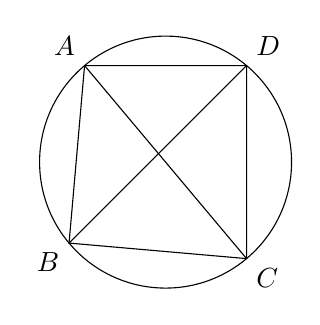
\begin{tikzpicture}[scale=0.8]
			\draw (0,0) circle (2cm);
			\coordinate (A) at (130:2);
            \coordinate (C) at (310:2);
            \coordinate (D) at (50:2); % Just random position for D
            \coordinate (B) at (220:2);
            \draw (A) -- (B) -- (C) -- (D) -- cycle;
            \draw (A) -- (C);
            \draw (B) -- (D);
			\node[above left] at (A) {$A$};
			\node[below left] at (B) {$B$};
			\node[below right] at (C) {$C$};
			\node[above right] at (D) {$D$};
		\end{tikzpicture}
		\end{center}
		Xét đường tròn ngoại tiếp tứ giác $ABCD$:
		\\
		1. Góc $\widehat{DBC}$ và góc $\widehat{DAC}$ cùng chắn cung $DC$.
		\[ \Rightarrow \widehat{DBC} = \widehat{DAC} = 40^\circ. \]
		2. Góc $\widehat{ABD}$ và góc $\widehat{ACD}$ cùng chắn cung $AD$.
		\[ \Rightarrow \widehat{ABD} = \widehat{ACD} = 35^\circ. \]
		Vậy $\widehat{DBC} = 40^\circ$ và $\widehat{ABD} = 35^\circ$.
	}
\end{bt}

%%%=============BT_3=============%%%
\begin{bt}%[9H3B7]
	Cho tứ giác $ABCD$ nội tiếp. Kéo dài cạnh $AB$ về phía $B$ một đoạn $BE$. Biết $\widehat{CBE} = 105^\circ$. Tính số đo góc $\widehat{ADC}$.
	\loigiai{
		\begin{center}
		\begin{tikzpicture}[scale=0.8]
			\draw (0,0) circle (2cm);
			\coordinate (A) at (140:2);
			\coordinate (D) at (40:2);
			\coordinate (C) at (-40:2);
			\coordinate (B) at (-140:2);
            \coordinate (E) at ($(A)!1.5!(B)$);
			\draw (A) -- (B) -- (C) -- (D) -- cycle;
            \draw (B) -- (E);
			\node[above left] at (A) {$A$};
			\node[below left] at (B) {$B$};
			\node[below right] at (C) {$C$};
			\node[above right] at (D) {$D$};
            \node[below] at (E) {$E$};
		\end{tikzpicture}
		\end{center}
		Ta có tứ giác $ABCD$ nội tiếp nên tổng hai góc đối $\widehat{ABC} + \widehat{ADC} = 180^\circ$.
		\\
		Mặt khác, $\widehat{ABC} + \widehat{CBE} = 180^\circ$ (hai góc kề bù).
		\\
		Suy ra $\widehat{ADC} = \widehat{CBE}$ (góc trong tại một đỉnh bằng góc ngoài tại đỉnh đối diện).
		\\
		Vậy $\widehat{ADC} = 105^\circ$.
	}
\end{bt}

%%%=============BT_4=============%%%
\begin{bt}%[9H3B7]
	Cho hình thang $ABCD$ ($AB \parallel CD$) nội tiếp đường tròn. Chứng minh $ABCD$ là hình thang cân và tính các góc của hình thang biết $\widehat{A} = 100^\circ$.
	\loigiai{
		\begin{center}
		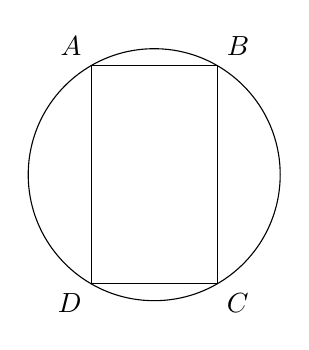
\begin{tikzpicture}[scale=0.8]
			\draw (0,0) circle (2cm);
            % Isos trapezoid.
			\coordinate (A) at (120:2);
			\coordinate (B) at (60:2);
			\coordinate (C) at (-60:2);
			\coordinate (D) at (-120:2);
			\draw (A) -- (B) -- (C) -- (D) -- cycle;
			\node[above left] at (A) {$A$};
			\node[above right] at (B) {$B$};
			\node[below right] at (C) {$C$};
			\node[below left] at (D) {$D$};
		\end{tikzpicture}
		\end{center}
		Do $AB \parallel CD$ nên bốn điểm $A, B, C, D$ cùng thuộc một đường tròn thì $ABCD$ phải là hình thang cân.
		\\
		(Hoặc: $AB \parallel CD \Rightarrow$ cung $AD$ = cung $BC \Rightarrow AD = BC \Rightarrow ABCD$ là hình thang cân).
		\\
		Vì $ABCD$ là hình thang cân nên $\widehat{B} = \widehat{A} = 100^\circ$.
		\\
		Tổng hai góc kề một cạnh bên của hình thang bằng $180^\circ$ (trong cùng phía):
		\[ \widehat{A} + \widehat{D} = 180^\circ \Rightarrow \widehat{D} = 180^\circ - 100^\circ = 80^\circ. \]
		Tương tự, $\widehat{C} = \widehat{D} = 80^\circ$.
		\\
		Vậy $\widehat{A} = \widehat{B} = 100^\circ$; $\widehat{C} = \widehat{D} = 80^\circ$.
	}
\end{bt}

%%%=============BT_5=============%%%
\begin{bt}%[9H3B7]
	Cho tứ giác $ABCD$ nội tiếp đường tròn $(O)$ có tia $AC$ là tia phân giác của góc $\widehat{BAD}$. Chứng minh $BC = CD$.
	\loigiai{
		\begin{center}
		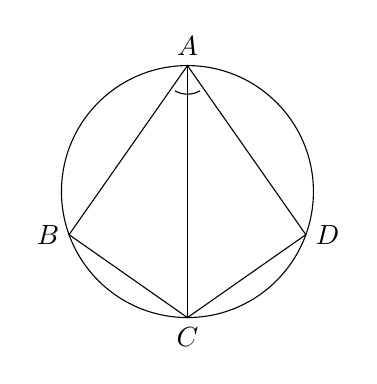
\begin{tikzpicture}[scale=0.8]
			\draw (0,0) circle (2cm);
			\coordinate (A) at (90:2);
            \coordinate (B) at (200:2);
            \coordinate (D) at (-20:2);
            \coordinate (C) at (270:2);
			\draw (A) -- (B) -- (C) -- (D) -- cycle;
            \draw (A) -- (C);
			\node[above] at (A) {$A$};
			\node[left] at (B) {$B$};
			\node[below] at (C) {$C$};
			\node[right] at (D) {$D$};
            \draw (A) ++(-0.2,-0.4) arc (240:270:0.4);
             \draw (A) ++(0.2,-0.4) arc (300:270:0.4); % Just marking visually
		\end{tikzpicture}
		\end{center}
		Ta có $AC$ là tia phân giác của góc $\widehat{BAD}$ nên $\widehat{BAC} = \widehat{DAC}$.
		\\
		Trong đường tròn ngoại tiếp tứ giác $ABCD$:
		\\
		- Góc $\widehat{BAC}$ chắn cung $BC$.
		\\
		- Góc $\widehat{DAC}$ chắn cung $DC$.
		\\
		Vì $\widehat{BAC} = \widehat{DAC}$ nên số đo cung $BC$ bằng số đo cung $DC$.
		\\
		Suy ra dây cung $BC$ bằng dây cung $DC$, hay $BC = CD$. (đpcm)
	}
\end{bt}
